\subsection{KNN Results}

For each movie, one of five CPU usage sequences is selected as query sequence and the rest four sequences are considered database (training) sequences, as described in \ref{sec:experimental_setup}, 
Then both query sequences and database sequences are divided into query subsequences and database subsequences with the same length.
For sequences with 1-second intervals, the length of subsequences $l$ is set to $l = [60, 120, 180, 300, 600]$, and each subsequence is extracted at every 20-second interval. 
For sequences with 5-second intervals, the length of subsequences $l$ is set to $l = [60, 120, 180, 300]$, and each subsequence is extracted at every 5-second interval. 

After building up query subsequences and database subsequences, we apply KNN method in order to classify each query subsequence based on database subsequences and predict the movie title of each subsequence. 
In this experiment, $k$ value is set to 3 since the maximum number of correct neighbors is 4. 
The prediction accuracy for each movie according to the length of query subsequences is shown in Table \ref{tab:knn_result}.
For all cases, it is clearly shown that the prediction accuracy increases as the length of query subsequences increases. 
A few movies (Movie \#1 and \#7 in \ref{tab:knn_interval1} and movie \#3 and \#7 in \ref{tab:knn_interval5}) show relatively low accuracy.
Especially, the prediction accuracy on movie \#7, \term{Mean Girls 2}, is the lowest in both 1-second and 5-second measurement interval.
We suppose that movie \#7 shows the lowest accuracy since the movie is a teenage movie with few action scenes and it is rather static.
However, we cannot assure since our experiment is performed only with 10 movies.

\begin{table}[!t]
\centering
\subtable[Measurement Interval = 1]{

\begin{tabular}{|c||>{\centering}m{0.7cm} | >{\centering}m{0.7cm} | >{\centering}m{0.7cm} | >{\centering}m{0.7cm} |c|}
\hline
\multirow{2}{*}{Movie ID} & \multicolumn{5}{c|}{Query Subsequence Length}	\\
\cline{2-6}
	& 60 & 120 & 180 & 300 & 600 \\
\hline
1	& 0.18	& 0.30	& 0.37	& 0.42	& 0.62		\\
2 	& 0.57	& 0.64	& 0.73	& 0.94	& 1.00		\\
3 	& 0.51	& 0.56	& 0.64	& 0.75	& 0.91		\\
4	& 0.53	& 0.67	& 0.79	& 0.93	& 1.00		\\
5	& 0.81	& 0.93	& 0.97	& 0.95	& 0.99		\\
6	& 0.83	& 0.95	& 0.97	& 0.98	& 1.00		\\
7 	& 0.27	& 0.30	& 0.38	& 0.46	& 0.58		\\
8 	& 0.66	& 0.84	& 0.89	& 0.99	& 1.00		\\
9 	& 0.54	& 0.77	& 0.89	& 0.97	& 0.99		\\
10 	& 0.50	& 0.79	& 0.91	& 0.95	& 1.00		\\	
\hline
\hline
Average & 0.54	& 0.68	& 0.77	& 0.83	& 0.91	 	\\
\hline
\end{tabular}
\label{tab:knn_interval1}
}
\subtable[Measurement Interval = 5]{

\begin{tabular}{|c||>{\centering}m{0.7cm} | >{\centering}m{0.7cm} | >{\centering}m{0.7cm} | >{\centering}m{0.7cm} |c|}
\hline
\multirow{2}{*}{Movie ID} & \multicolumn{5}{c|}{Query Subsequence Length}	\\
\cline{2-6}
	& 60 & 120 & 180 & 300 & 600			\\
\hline
1	& 0.51	& 0.87	& 0.94	& 0.99 & 1.00	\\
2 	& 0.63	& 0.83	& 0.92	& 0.95 & 0.98	\\
3 	& 0.30	& 0.60	& 0.73	& 0.89 & 1.00	\\
4	& 0.53	& 0.82	& 0.94	& 1.00 & 1.00	\\
5	& 0.47	& 0.76	& 0.88	& 0.94 & 1.00	\\
6	& 0.49	& 0.83	& 0.96	& 1.00 & 1.00	\\
7 	& 0.19	& 0.43	& 0.63	& 0.85 & 0.99	\\
8 	& 0.50	& 0.88	& 0.97 & 1.00 & 1.00	\\
9 	& 0.47	& 0.86	& 0.95	& 0.97 & 0.98	\\
10 	& 0.49	& 0.82	& 0.92	& 1.00 & 1.00	\\	
\hline
\hline
Average & 0.46	& 0.77	& 0.88 & 0.96 & 0.99 	\\
\hline
\end{tabular}
\label{tab:knn_interval5}
}
\caption{Success Rate of Prediction: KNN}
\label{tab:knn_result}
\end{table}

The overall prediction accuracy according to the length of query subsequences is shown in Figure \ref{fig:knn_result}.
This experimental result shows that given 10 movies and their CPU usage statistics of 300 seconds with 1-second measurement interval or of 180 seconds with 5-second measurement interval, our side channel attack algorithm predicts which movie a user is watching at the accuracy of higher than 80$\%$.
The accuracy with 5-second measurement interval is usually higher than the accuracy with 1-second measurement interval, since the former contains less noise due to the effect of averaging over the period of 5 seconds. 
However, when the query subsequence length is set to 60-second, the prediction accuracy with 5-second measurement interval is as low as 46\%, which is lower than the accuracy with 1-second measurement interval, 54\%. 
In case of 5-second measurement interval, a query subsequence with 60-second length contains only 12 measurement results in it. 
If we consider each query subsequence a vector with 12 elements, we suppose that the length of vectors is too short to calculate Euclidean distance between two vectors stably. 


\begin{figure}[!t]
\centering
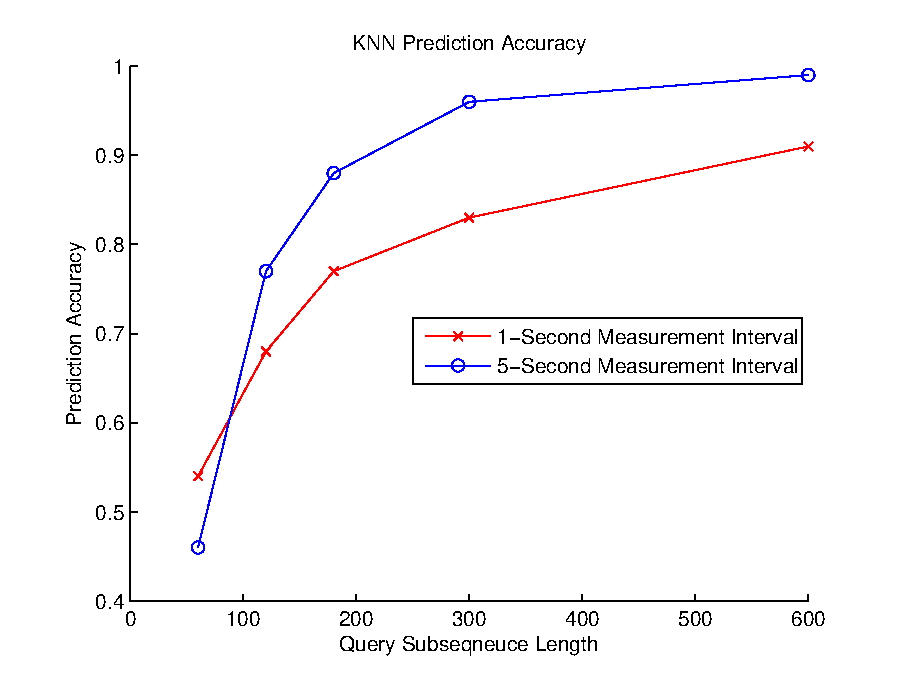
\includegraphics[scale=0.40]{Figures/knn_result}
\caption{KNN Prediction Accuracy}
\label{fig:knn_result}
\vspace{-5mm}
\end{figure}